\documentclass{article}
\usepackage{graphicx} % Required for inserting images
\usepackage{float}
\usepackage{subcaption}
\title{Misure di densità}
\author{Alessandro Di Meglio\\Francesco Angelo Fabiano Antonacci}
\date{\today} 



\begin{document}

\maketitle{}


\section{Scopo dell'esperienza}
Il primo scopo dell'esperienza è quello di misurare la densità dell'ottone, dell'alluminio,dell'acciaio.
Il secondo scopo dell'esperienza è quello di verificare la dipendenza cubica della massa dal raggio.

\section{Cenni teorici}
La densità di un corpo è definita dalla seguente equazione:
\begin{equation}
\rho = \frac{m}{V}
\end{equation}
dove m è la massa e V è il volume.
Ci si aspetta che il fit con l'equazione (1) delle misure che verranno fatte sia una linea retta passante per l'origine.

La massa di una sfera dipende cubicamente dal suo raggio. Nell'esperienza, per  considerazioni che verranno, fatte verrà usato:
\begin{equation}
r=km^\frac{1}{3}
\end{equation}


\section{Apparato strumentale}
Gli strumenti utilizzati per l'esperienza sono:

\subsection{Strumenti per la misurazione di lunghezze}
\begin{itemize}
\item \textbf{Calibro ventesimale}  con risoluzione di 0.05mm
\item \textbf{Calibro cinquantesimale} con risoluzione di 0.02mm
\item \textbf{Calibro Palmer} con risoluzione di 0.01mm
\end{itemize}
\subsection{Strumenti per la misurazione delle masse}

\begin{itemize}
\item \textbf{Bilancia di precisione} con risoluzione di 1mg
\end{itemize}



\subsection{Corpi}
I corpi su cui sono state fatte le misure, divisi per materiale, sono i seguenti: 
\subsubsection{\textbf{Alluminio}}

\begin{itemize}
\item 2 parallelepipedi 
\item 2 cilindri 
\end{itemize}

\subsubsection{Ottone}

\begin{itemize}
\item  2 cilindri
\item 1 parallelepipedo a base esagonale
\item 1 parallelepipedo a base rettangolare
\end{itemize}

\subsubsection{Acciaio}

\begin{itemize}
\item 5 sfere
\end{itemize}


\section{Descrizione delle misure}
Per quasi tutte le misurazioni di lunghezza effettuate, si è utilizzato il calibro Palmer. Solo due misure sono state effettuate con il calibro cinquantesimale in quanto la lunghezza da effettuare era maggiore della misura massima misurabile dal calibro Palmer. Le due misure in questione sono l'altezza di un cilindro e di un parallelepipedo entrambi di ottone.
Riportiamo con una tabella le misure effettuate:
\subsection{Dati delle misurazioni dei corpi di alluminio}
\begin{table}[H]
    \centering
    \begin{tabular}{|c|c|c|c|c|}
        \hline
        Corpo & Massa [g]& Lato 1 [mm] & Lato 2 [mm] & Lato 3 [mm] \\
        \hline
        Parallelepipedo 1 & $4.853 \pm 0.001$ & $10.05 \pm 0.01$ & $10.04 \pm 0.01$ &  $18.43 \pm 0.01$ \\
        Parallelepipedo 2 & $7.766 \pm 0.001$ & $8.14 \pm 0.01$ & $17.78 \pm 0.01$ &  $20.07 \pm 0.01$ \\
        Cilindro 1 & $5.789 \pm 0.001$ & $11.96 \pm 0.01$ & $19.08 \pm 0.01$ & \\
        Cilindro 2 & $15.777 \pm 0.001$ & $18.91 \pm 0.01$ & $19.80 \pm 0.01$ & \\
        \hline
    \end{tabular}
    \caption{Tabella con i dati dei corpi}
    \label{tab:dati_corpi}
\end{table}
\subsection{Dati delle misurazioni delle corpi di ottone}



\begin{table}[H]
    \centering
    \begin{tabular}{|c|c|c|c|c|}
        \hline
        Corpo & Massa [g] & Lato 1 [mm]& Lato 2 [mm] & Lato 3 [mm] \\
        \hline
        Cilindro 1 & $10.764 \pm 0.001$ & $9.96 \pm 0.01$ & $16.41 \pm 0.01$ & \\
        Cilindro 2 & $24.528 \pm 0.001$ & $9.96 \pm 0.01$ & $37.30 \pm 0.02$ & \\
        Parallelepipedo & $34.725 \pm 0.001$ & $9.98 \pm 0.01$ & $9.95 \pm 0.01$ & $41.50 \pm 0.02$ \\
        Parallelepipedo a base esagonale & $16.474 \pm 0.001$ & $9.94 \pm 0.01$ & $22.82 \pm 0.01$ & \\
        \hline
    \end{tabular}
    \caption{Tabella con i dati dei corpi. Nota:con Lato1 per il parallelepipedo a base esagonale si intende l'apotema }
    \label{tab:dati_corpi_aggiornati}
\end{table}
\subsection{Dati delle misurazioni delle corpi in acciaio}
\begin{table}[H]
    \centering
    \begin{tabular}{|c|c|c|}
        \hline
        Nome & Massa[g] & Raggio [mm] \\
        \hline
        Sfera 1 & $3.524 \pm 0.001$ & $9.52 \pm 0.01$ \\
        Sfera 2 & $8.359 \pm 0.001$ & $12.69 \pm 0.01$ \\
        Sfera 3 & $11.889 \pm 0.001$ & $14.27 \pm 0.01$ \\
        Sfera 4 & $28.193 \pm 0.001$ & $19.03 \pm 0.01$ \\
        Sfera 5 & $44.821 \pm 0.001$ & $22.20 \pm 0.01$ \\
        \hline
    \end{tabular}
    \caption{Tabella con gli ultimi dati delle sfere}
    \label{tab:dati_sfere}
\end{table}





\section{Analisi dei dati}


\subsection{Misure di densità}
E' stata usata una legge lineare per fare il fit delle misure prese.
E' stato scelto di usare come grandezza con incertezza trascurabile la massa in quanto per utilizzare la funzione di python $curve\_fit()$ è necessario che sia verificata la seguente relazione:
\begin{equation}
\sigma r \gg \left|{ \frac{dr}{dm}}\right| \sigma m
\end{equation}
Dove r è il raggio e m la massa.
La relazione è verificata per un ordine di grandezza sui solidi di alluminio, segue che è verificata per tutti i solidi.
L'algoritmo di best-fit ha restituito un coefficiente w e un' intercetta q per ogni legge lineare.
Li riportiamo in tabella.
\begin{table}[H]
    \centering
    \begin{tabular}{|c|c|c|c|}
        \hline
        Materiale &$ \rho[kg/m^3]$ &$w [m^3/mg]$&$ q [m^3/mg]$ \\
        \hline
        Alluminio & $2946 \pm 46$ & $ 339\pm 5$ &$0.22\pm 0.05$\\
        Acciaio & $7824 \pm 4$ & $130.0 \pm0.6$ & $0.002\pm0.001$ \\
        Ottone & $8229\pm 398$ &  $121\pm 6$ &$ -0.1\pm0.1 $\\

        \hline
    \end{tabular}
    \caption{Densità calcolate dai dati}
    \label{tab:dati_sfere}
\end{table}
Il coefficiente w, essendo il reciproco della densità, è  stato utilizzato per calcolarla e stimarne l'errore.
L'intercetta q è un parametro di controllo:idealmente, per quanto accennato in \textbf{Cenni Teorici} dovrebbe essere 0.
Il fatto che ciascuna delle intercette sia minore dell'errore di misura della massa è una verifica delle misure e dell'analisi dei dati, che pur non ne conferma la correttezza.


\begin{figure}
\centering
		\begin{subfigure}{0.4\textwidth}
   			 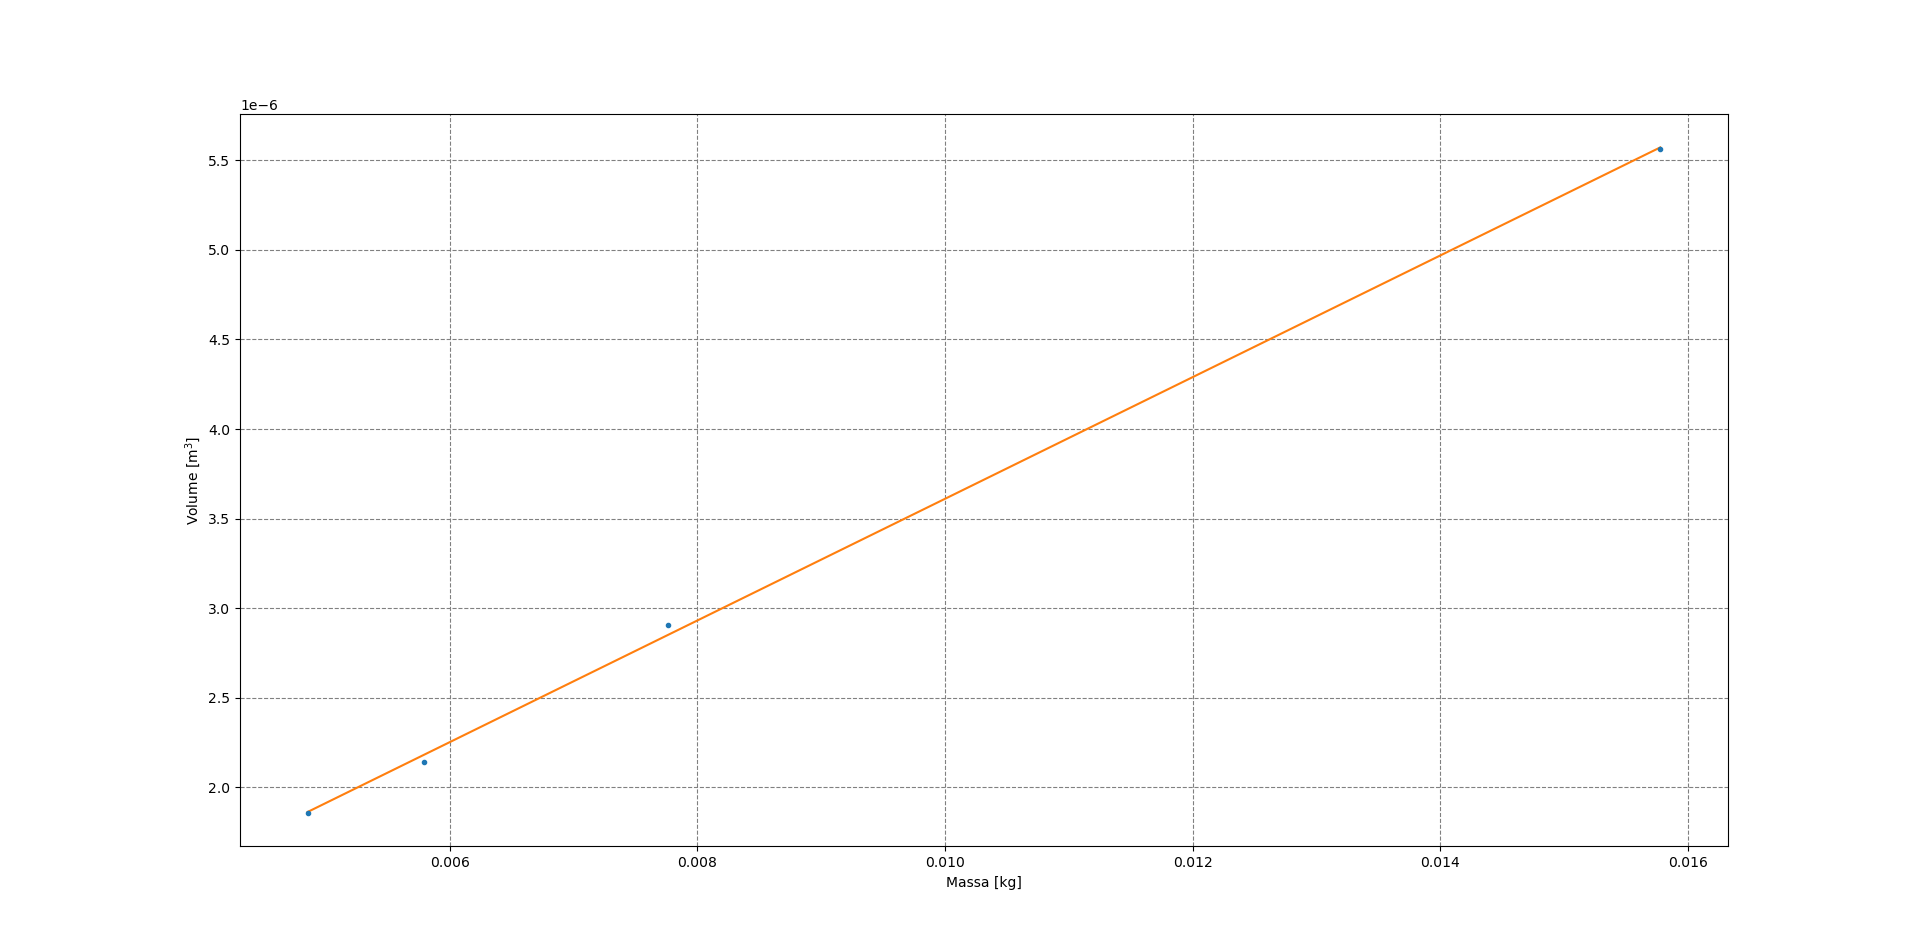
\includegraphics[width=\textwidth]{Grafico_massa-volume_Alluminio.png}
    				\caption{Grafico massa volume Alluminio}
   			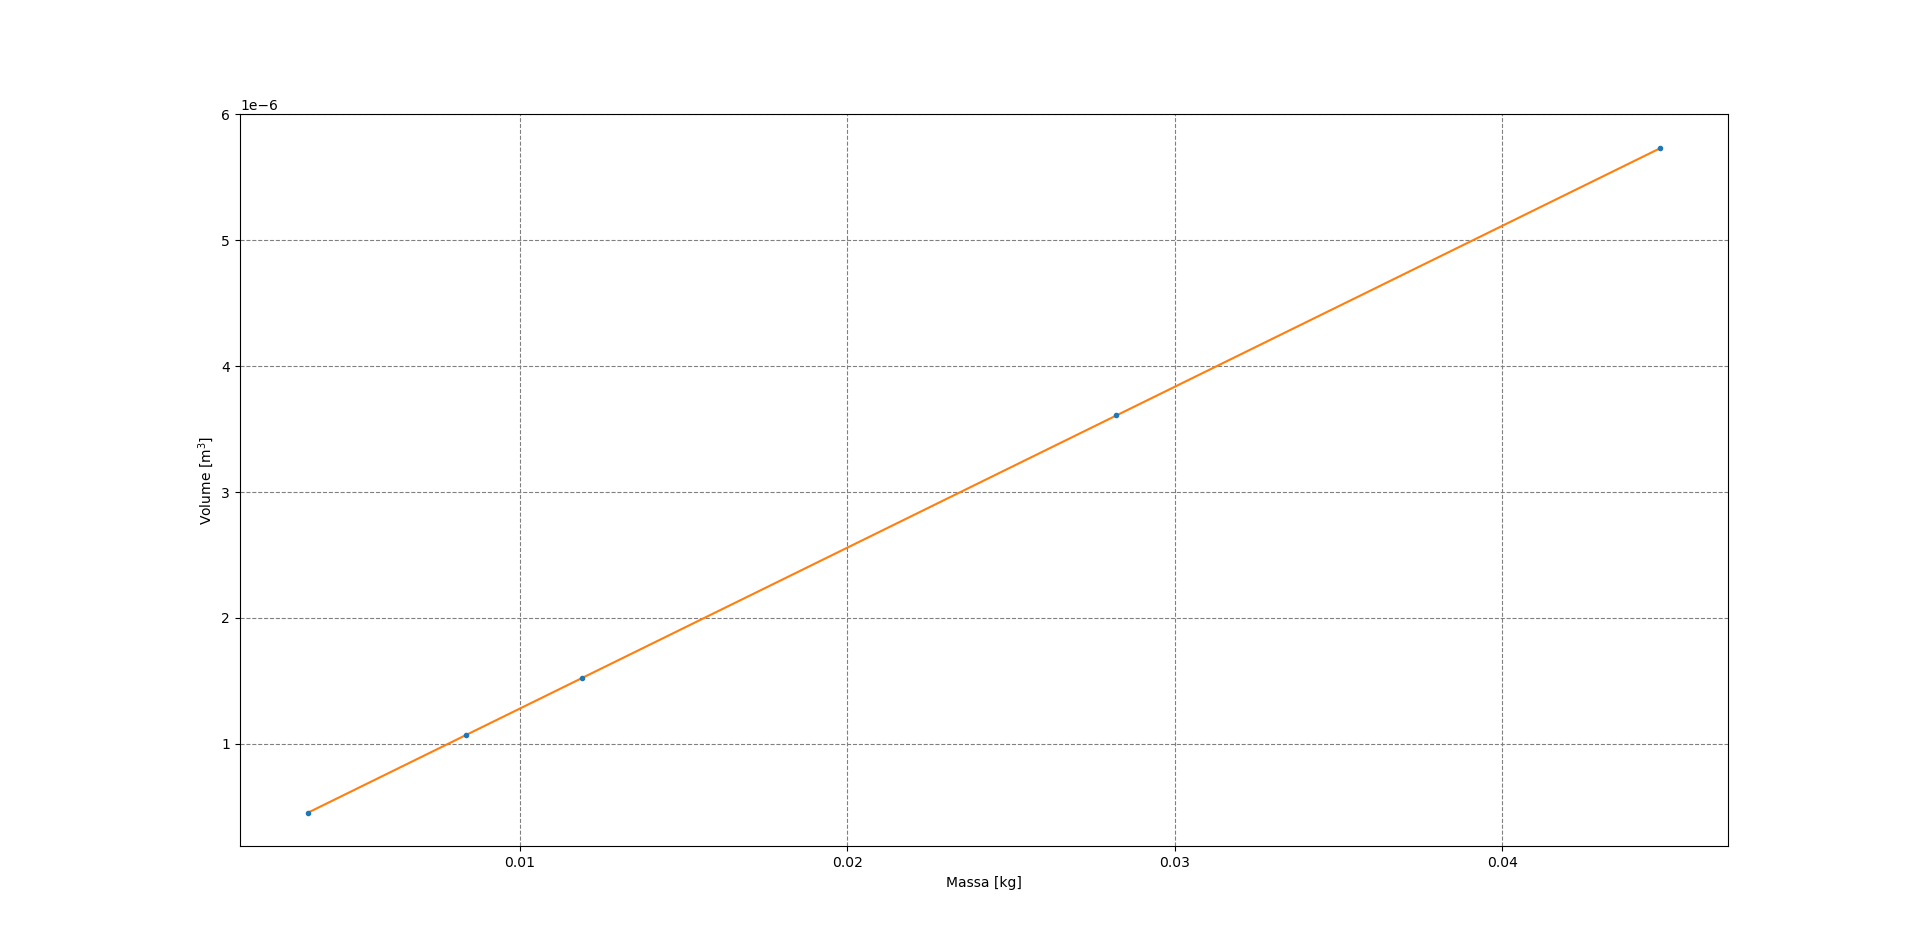
\includegraphics[width=\textwidth]{Grafico_massa-volume_Acciaio.png}
   				 \caption{Grafico massa volume Acciaio}
			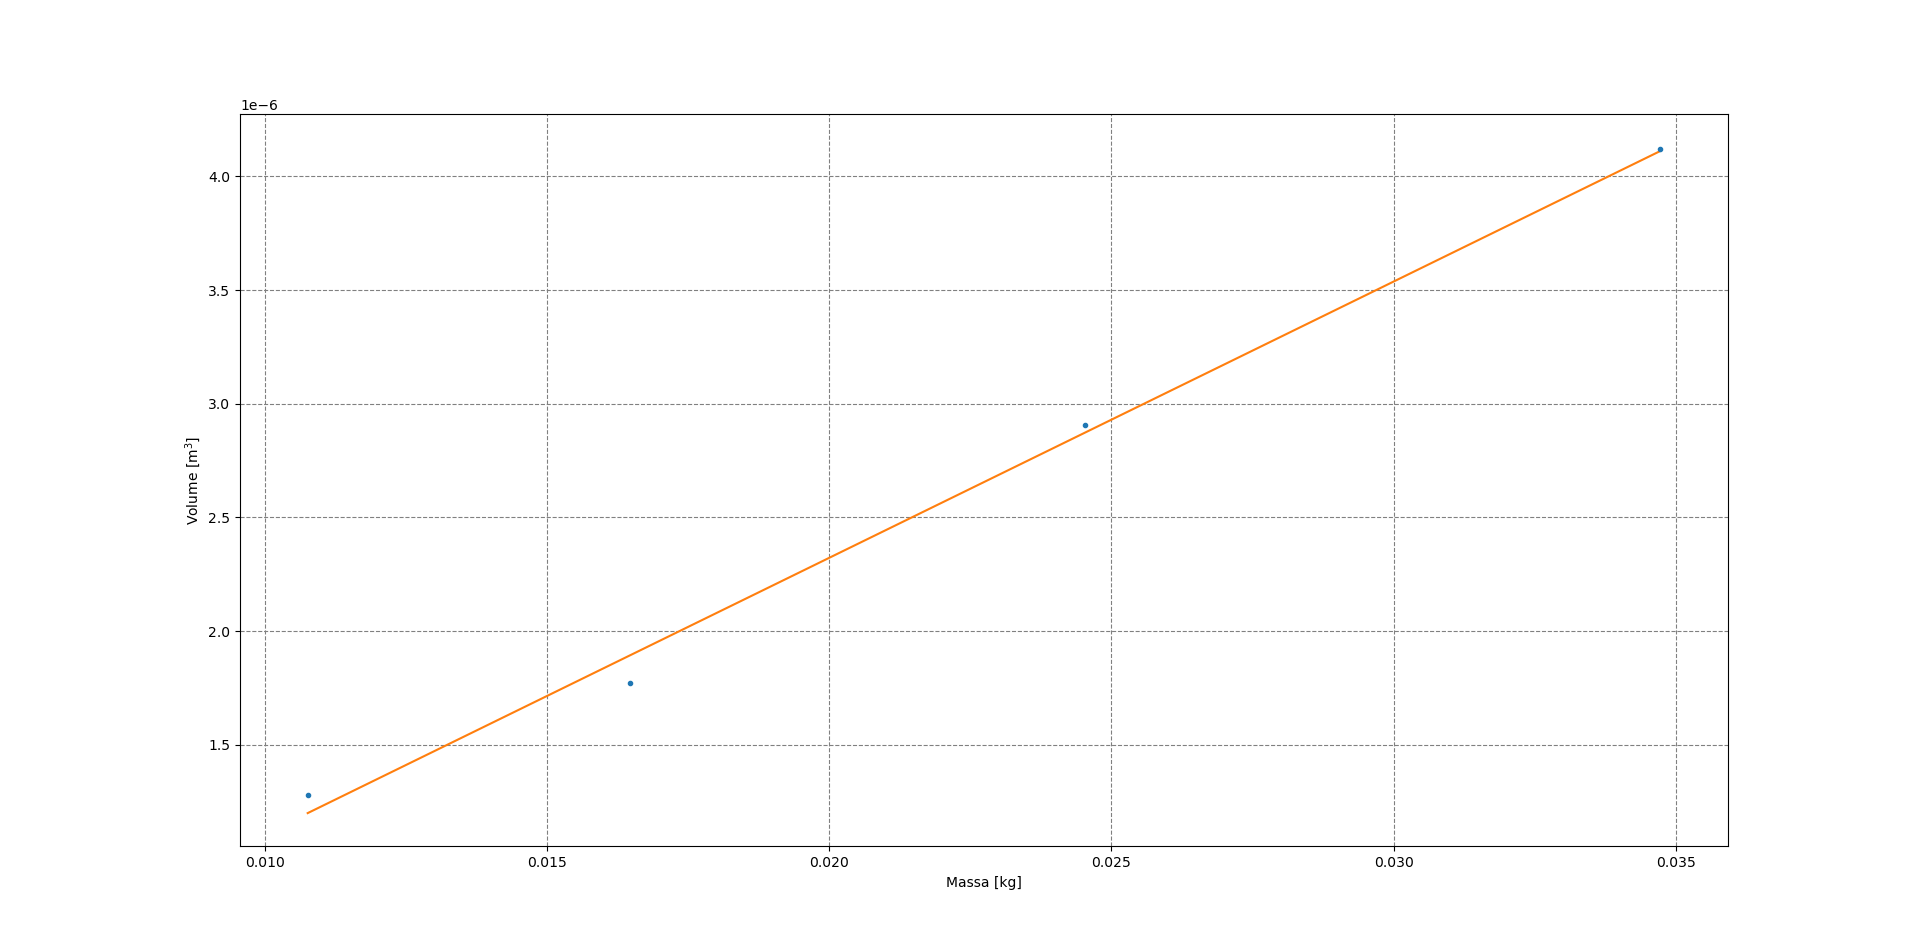
\includegraphics[width=\textwidth]{Grafico_massa-volume_Ottone.png}
   				 \caption{Grafico massa volume Ottone}
			
		\end{subfigure}
		\begin{subfigure}{0.4\textwidth}   
			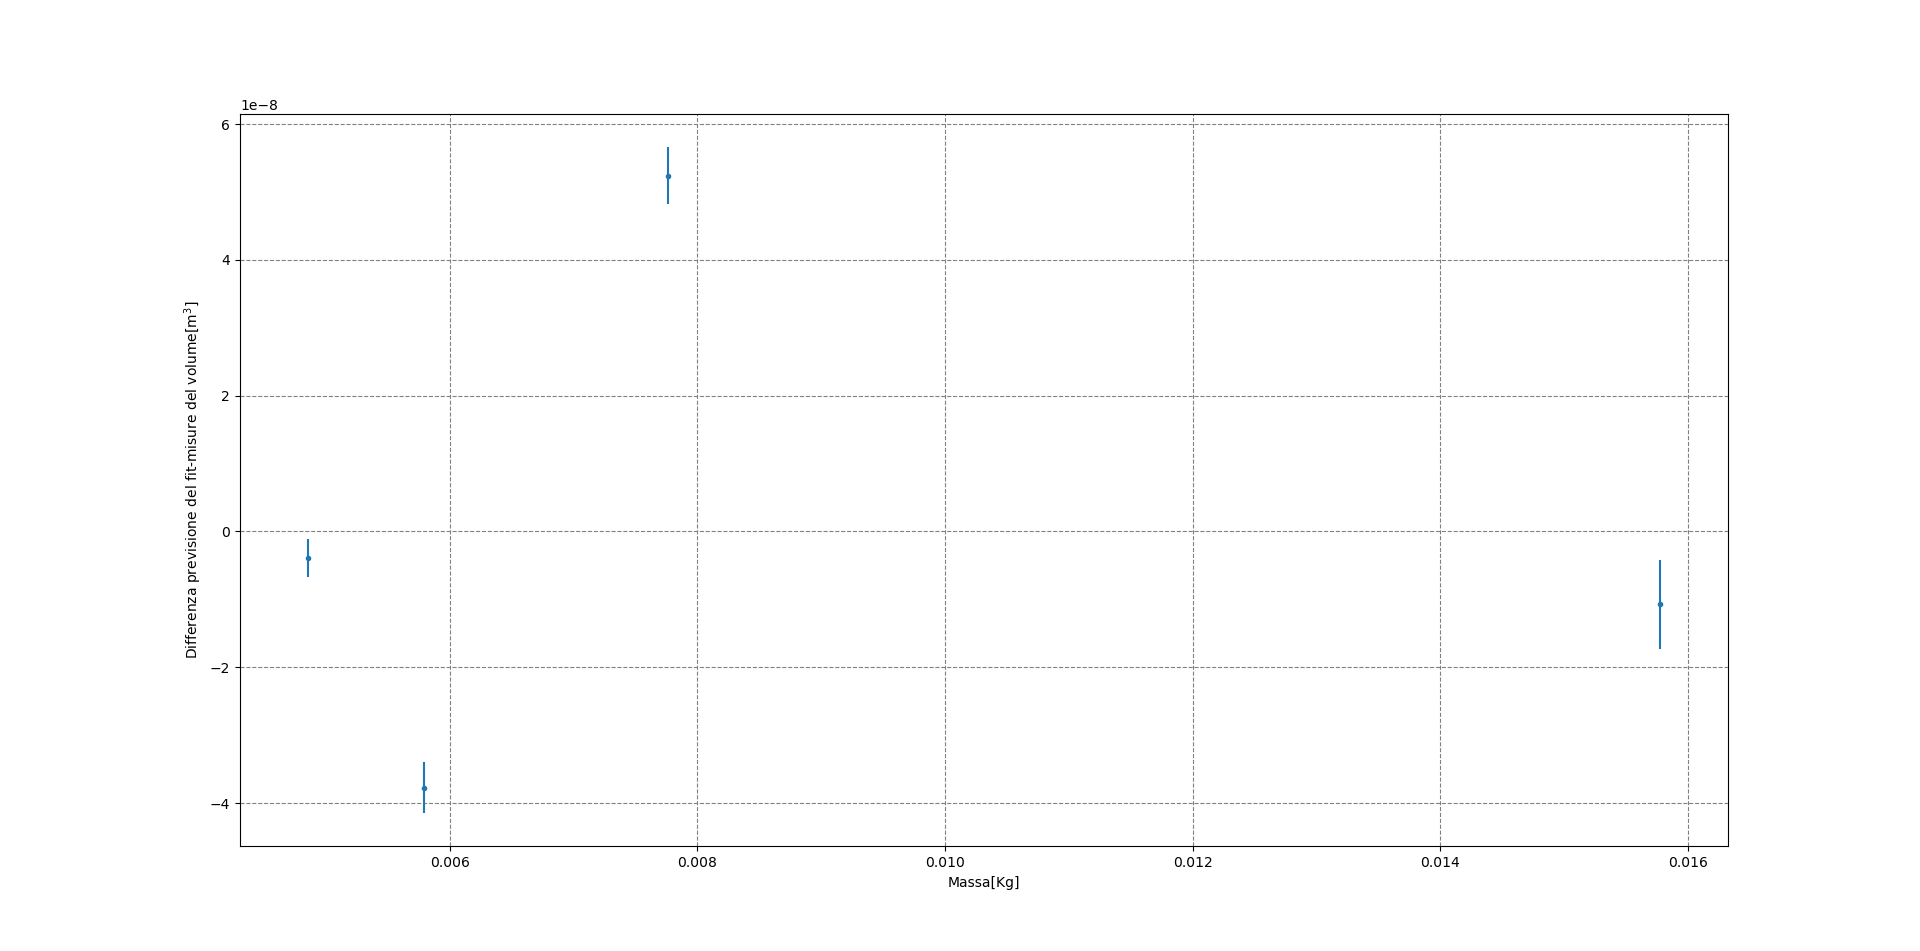
\includegraphics[width=\textwidth]{Grafico_dei_residui_dei_solidi_di_alluminio.png}
    				\caption{Grafico dei residui Alluminio}
			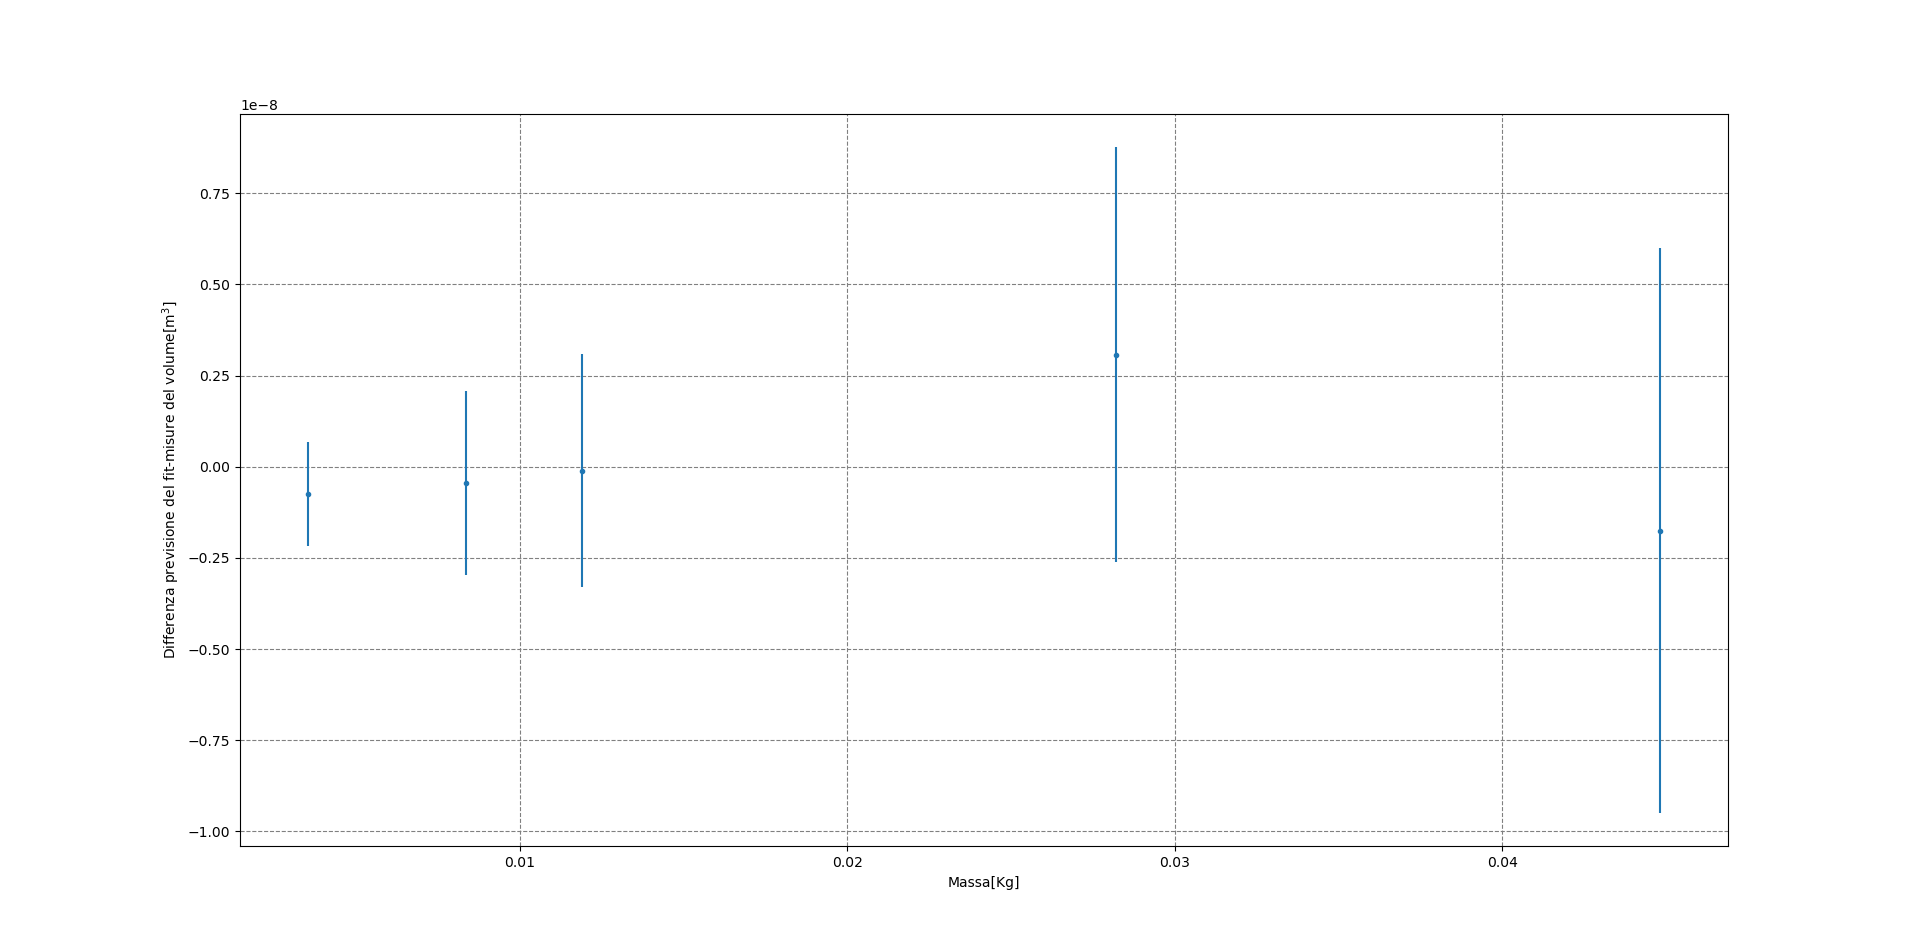
\includegraphics[width=\textwidth]{Grafico_dei_residui_dei_solidi_di_acciaio.png}
   				 \caption{Grafico dei residui Acciaio}
			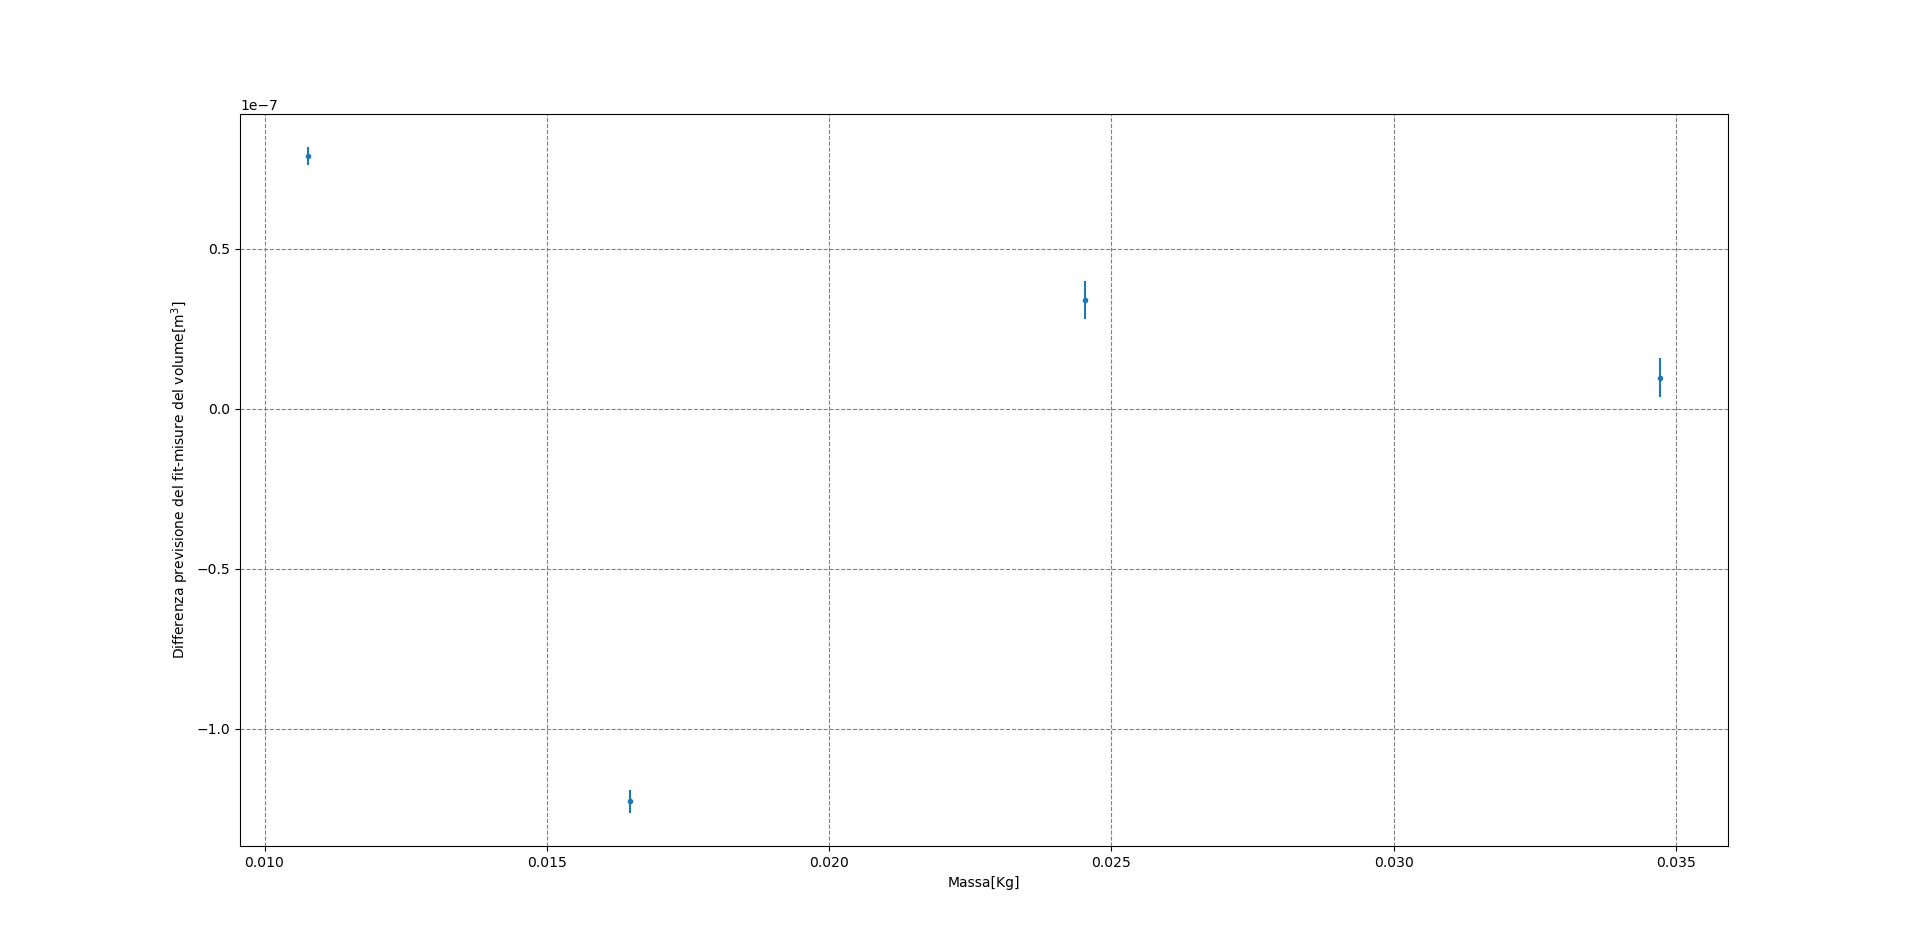
\includegraphics[width=\textwidth]{Grafico_dei_residui_dei_solidi_di_ottone.png}
   				 \caption{Grafico dei residui Ottone}
		\end{subfigure}
   


\end{figure}



\subsection{Verifica legge di potenza}
Anche per la verifica della legge di potenza è stato usata la funzione $curve\_fit$ ed è stata scelta la massa come grandezza con l'errore di misura trascurabile.
Si è  osservato che la massa più piccola soddisfa la relazione (3) in quanto il termine a sinistra è maggiore di due ordini di grandezza  ; 
le altre masse hanno un valore  minore della derivata nel punto: segue che anch'esse  rispettano la relazione.
L'algoritmo di best fit ha restituito i seguenti valori:
\begin{table}[H]
    \centering
    \begin{tabular}{|c|c|}
        \hline
        $k[m^3/kg]$ & $esponente$ \\
        \hline
       $ 0.03122\pm0.0001 $ & $0.3330\pm0.0001$\\

        \hline
    \end{tabular}
    
\end{table}



\begin{figure}
	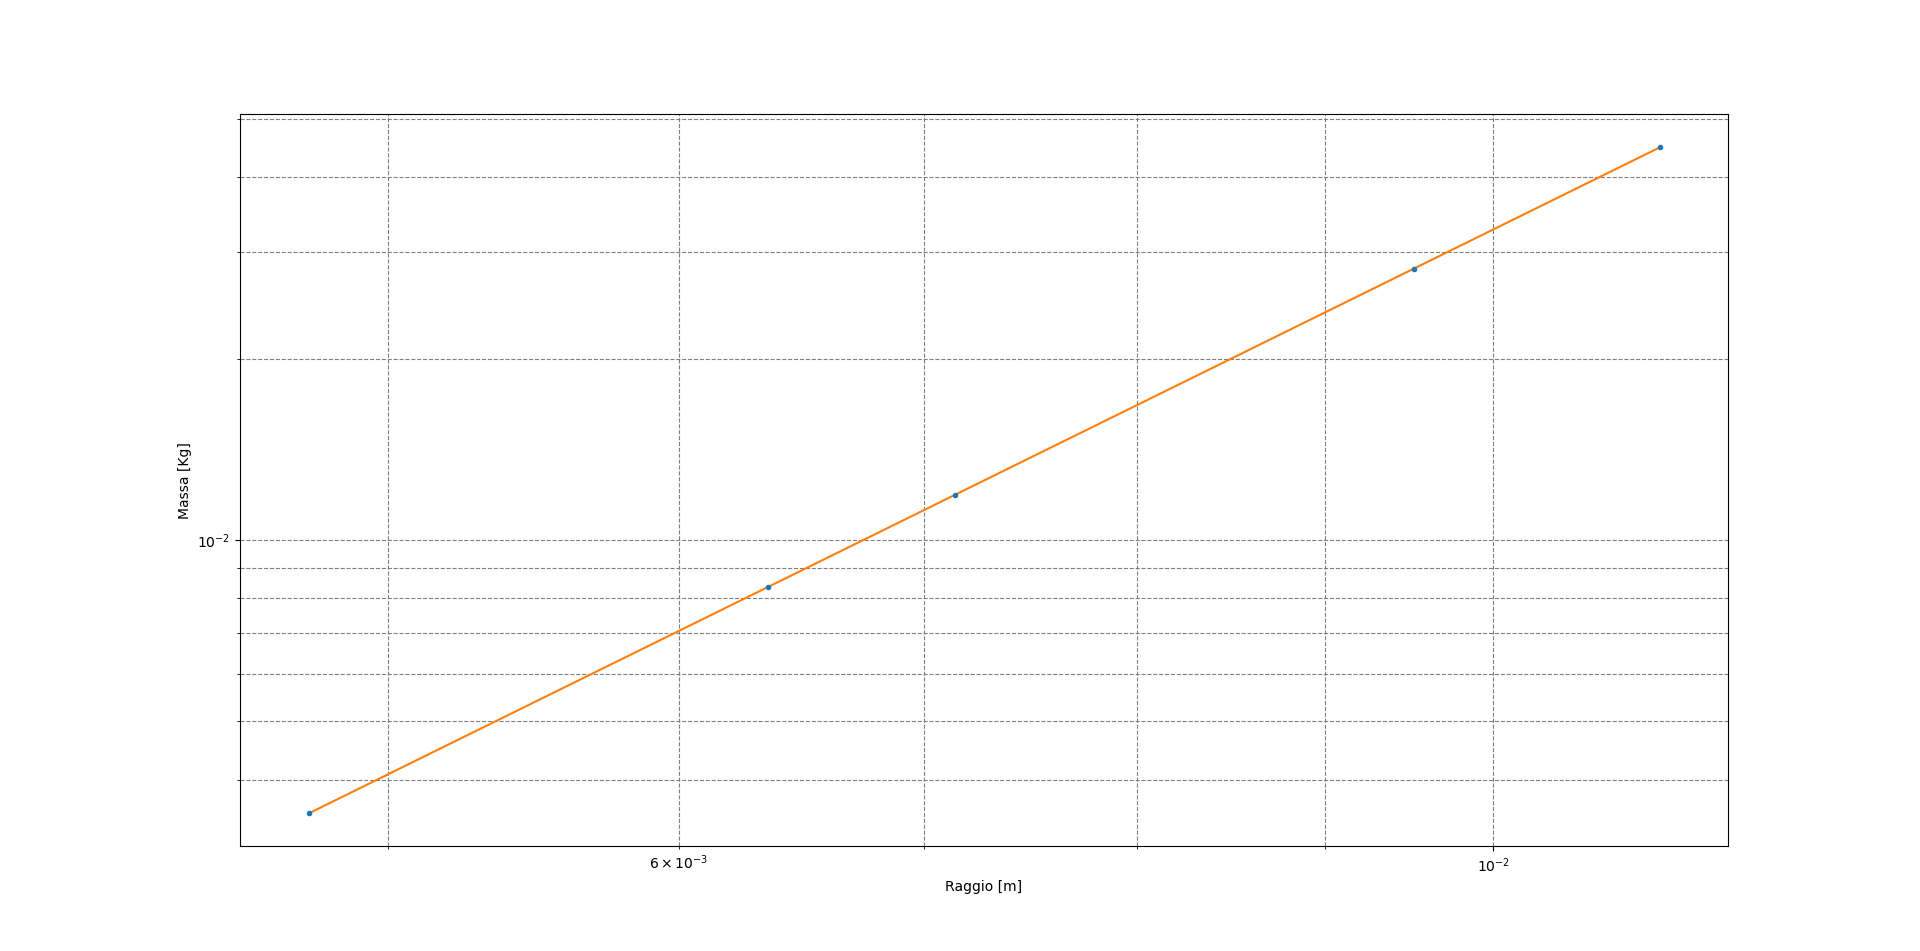
\includegraphics[width=\textwidth]{Grafico_massa-raggio.png}
		\caption{Grafico massa raggio per le sfere di acciaio}
\end{figure}

\section{Conclusioni}
\subsection{Misure di densità}
I valori ricavati in quest'esperienza sono distanti al più una barra d'errore con quelli tabulati forniti.

\begin{table}[H]
    \centering

    \begin{tabular}{|c|c|c|}
        \hline
        Materiale &$ \rho_{misurata}[kg/m^3]$ &$\rho_{tabulata}[kg/m^3]$ \\
        \hline
        Alluminio & $2946\pm46$ & $2710$ \\
        Acciaio & $7824\pm4$ & $7480–8000$ \\
        Ottone & $8229\pm398$ &  $8400–8700$  \\

        \hline
    \end{tabular}
    \caption{I valori riportati non hanno l'errore specificato: si assume che sia sull'ultima cifra significativa.}
    \label{tab:dati_sfere}
\end{table}

\subsection{Verifica legge di potenza}
La legge di potenza è verificata: l'esponente si trova a tre barre di errore da$\frac{1}{3}$ , il valore previsto.
Il valore previsto del coefficiente è: 
\begin{equation}
 k_{exp}=(\frac{3}{4\rho_{acciaio}\pi})^{esponente}=0.03125[m^3/kg]
\end{equation}

Il valore stimato dal fit è a tre barre di errore.


\begin{figure}
	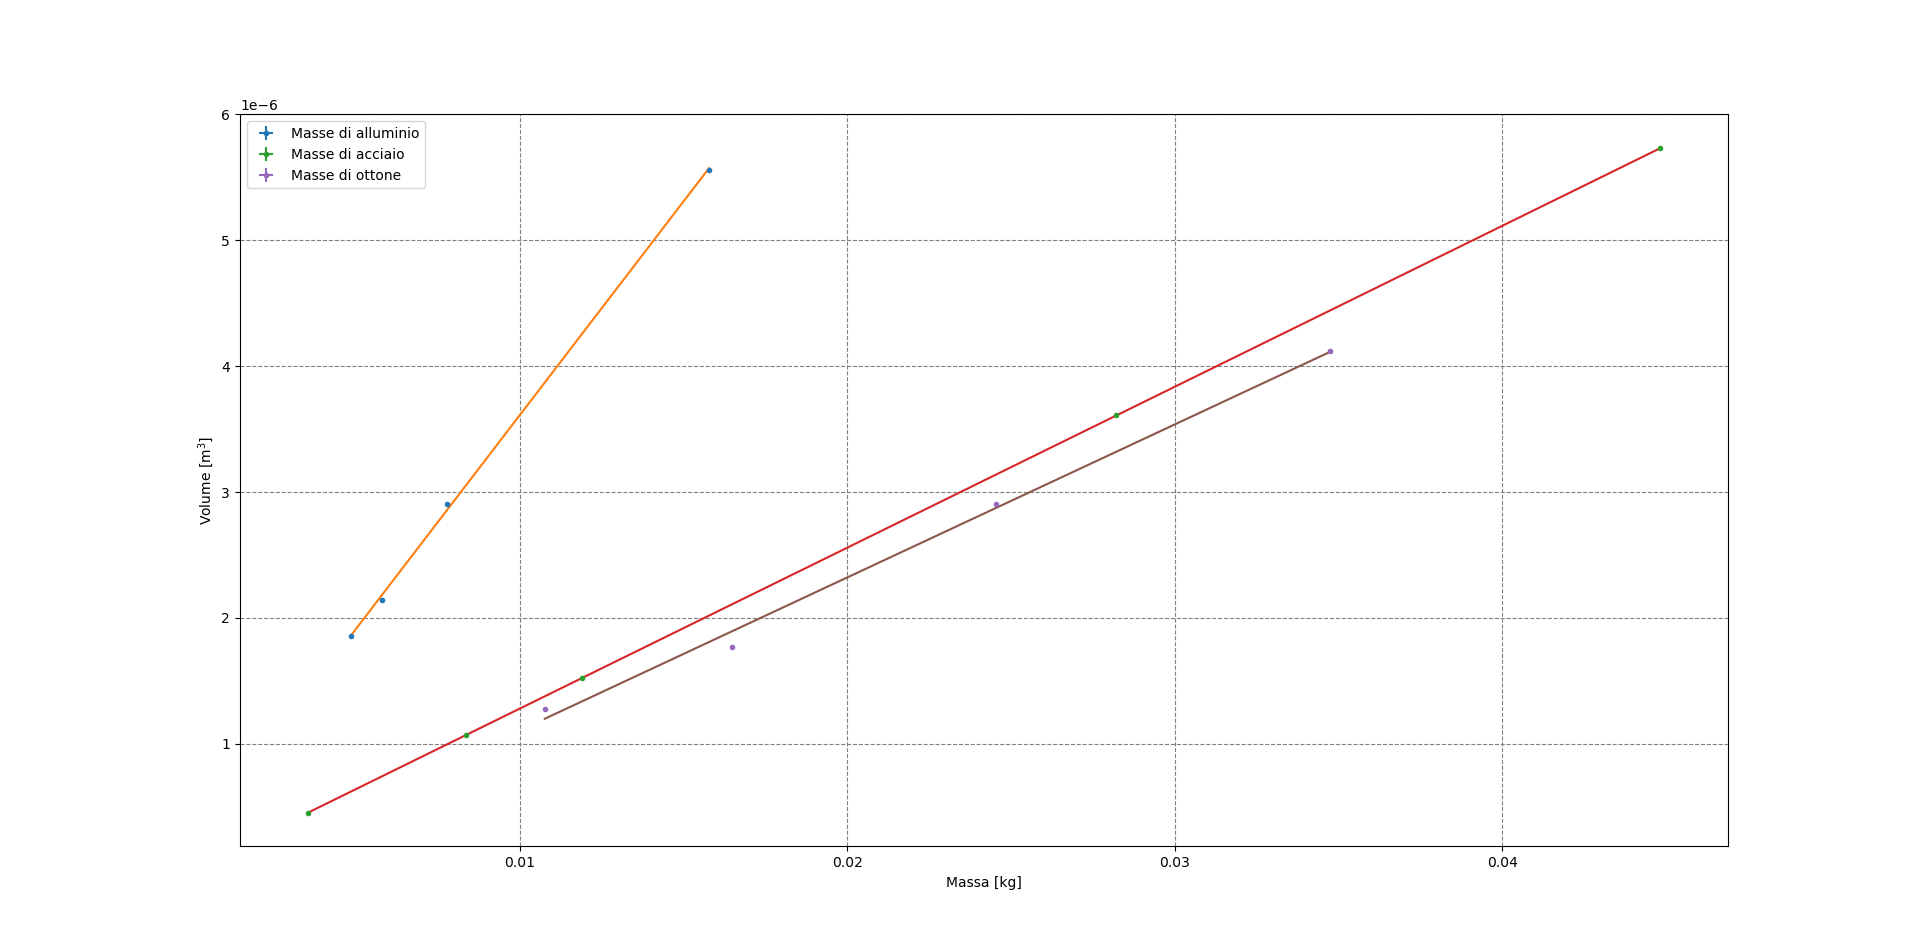
\includegraphics[width=\textwidth]{Grafico_unificato.png}
		\caption{Grafico massa volume unificato}
\end{figure}




\end{document}